% !TeX root = RJwrapper.tex
\title{\pkg{rbw}: An R Package for Constructing Residual Balancing
Weights}
\author{by Derick S. Baum and Xiang Zhou}

\maketitle

\abstract{%
We describe the R package \CRANpkg{rbw}, which implements the method of
residual balancing weights (RBW) for estimating marginal structural
models. In contrast to other methods such as inverse probability
weighting (IPW) and covariate balancing propensity scores (CBPS), RBW
involves modeling the conditional means of post-treatment confounders
instead of the conditional distributions of the treatment to construct
the weights. RBW is thus easier to use with continuous treatments, and
the method is less susceptible to model misspecification issues that
often arise when modeling the conditional distributions of treatments.
RBW is also advantageous from a computational perspective. As its
weighting procedure involves a convex optimization problem, RBW
typically locates a solution considerably faster than other methods
whose optimization relies on nonconvex loss functions --- such as the
recently proposed nonparametric version of CBPS. We explain the
rationale behind RBW, describe the functions in \CRANpkg{rbw}, and then
use real-world data to illustrate their applications in three scenarios:
effect estimation for point treatments, causal mediation analysis, and
effect estimation for time-varying treatments with time-varying
confounders.
}

\hypertarget{intro}{%
\section{Introduction}\label{intro}}

This paper describes the R package \CRANpkg{rbw}, which implements the
method of residual balancing weights for estimating marginal structural
models (MSMs) \citep{zhouResidualBalancingMethod2020a}. MSMs seek to
estimate causal effects in the presence of post-treatment confounding
--- a common issue in the social sciences. In studies of time-varying
treatments, prior treatments may affect the confounders of future
treatments. For example, research has shown that political candidates'
decision to run negative advertisements is shaped by their positions in
recent polling data, which are in turn affected by their previous
decisions to run negative advertisements
\citep{lauEffectsNegativePolitical2007, blackwellFrameworkDynamicCausal2013}.
Post-treatment confounding can also occur in causal mediation analysis
when confounders of the mediator-outcome relationship are affected by
the treatment. For example, such a problem arises in a study of the
mediating role of morality in the effect of shared democracy on public
support for war \citep{tomzPublicOpinionDemocratic2013a}. Post-treatment
variables, such as respondents' beliefs about the likelihood of victory,
may affect both perceptions of morality and support for military
intervention.

MSMs aim to address two types of bias associated with conventional
regression methods that adjust naively for post-treatment confounders:
overcontrol and collider-stratification bias
\citetext{\citealp{robinsNewApproachCausal1986}; \citeyear{robinsMarginalStructuralModels2000a}}.
Conditioning naively on post-treatment confounders can create
overcontrol bias as it blocks the effect of the treatment on the outcome
that passes through these variables. Additionally, it can lead to
collider-stratification bias when post-treatment confounders are
affected by unobserved determinants of the outcome. This is because the
adjustment will create a spurious association between the treatment and
the unobserved variables.

Researchers often use inverse probability weighting (IPW) to fit MSMs
\citep[for an in-depth exposition of the method,
see][]{robinsMarginalStructuralModels2000, robinsMarginalStructuralModels2000a, coleConstructingInverseProbability2008a}.
In longitudinal settings, MSMs with IPW involve fitting a model for the
conditional mean of the outcome given the treatment history using
weights that break the dependence between past confounders and the
treatment at each time point. In essence, the weights create a
pseudo-population where the marginal mean of the potential outcomes
under a treatment history equals the conditional mean of the observed
outcome given the treatment history. The R package \CRANpkg{ipw}
provides functions for estimating inverse probability weights
\citep{vanderwalIpwPackageInverse2011, R-ipw}.

However, IPW's success depends on correct specification of the models
for the conditional distributions of exposure to treatment and/or
mediator (hereafter jointly referred to as ``exposures''), which is
difficult to achieve in practice. Moreover, even when these models are
correctly specified, IPW is inefficient and susceptible to finite-sample
bias
\citep{zhouResidualBalancingMethod2020a, wangDiagnosingBiasInverse2006}.
Finally, when the exposures are continuous, IPW may perform poorly due
to unreliable estimation of conditional densities
\citep{naimiConstructingInverseProbability2014, vansteelandtEstimatingDirectEffects2009}.

Alternative methods have attempted to mitigate these shortcomings. In
particular, Imai and Ratkovic's
\citetext{\citeyear{imaiCovariateBalancingPropensity2014}; \citeyear{imaiRobustEstimationInverse2015}}
covariate balancing propensity score (CBPS) method proposes a set of
balancing conditions when estimating the propensity scores. Because it
seeks to maximize the covariate balance between the treatment and
control groups, this method is less sensitive to model misspecification
than IPW. \citet{fongCovariateBalancingPropensity2018} expand CBPS to
accommodate continuous exposures, but the challenges involved in
modeling conditional densities persist. With this in mind, they have
also developed a nonparametric extension that constructs weights that
maximize the empirical likelihood while meeting a set of balancing
conditions. Though the nonparametric CBPS (npCBPS) circumvents the need
for specifying a functional form for the propensity score, it does so at
a cost: since the empirical likelihood is not generally convex, the
optimization procedure is often slow and may fail to find a solution.
The latter can happen, for example, when we have a large number of
covariates. The authors advance a workaround that adds flexibility to
the covariate balancing conditions and penalizes the remaining
imbalance. In doing so, they ensure that a weighting solution exists.
Users can implement CBPS in R with the \CRANpkg{CBPS} package
\citep{R-CBPS}.

Recently, \citet{zhouResidualBalancingMethod2020a} propose the method of
residual balancing weights (RBW) for estimating MSMs. RBW involves
fitting models for the conditional means of post-treatment confounders
given past treatments and confounders and extracting their residual
terms. It then uses Hainmueller's
\citeyearpar{hainmuellerEntropyBalancingCausal2012} entropy balancing
method to find weights such that, in the weighted sample, 1) the
residuals are orthogonal to future exposures, past treatments, and past
confounders, and 2) the relative entropy between the weights and a set
of base weights (e.g., survey sampling weights) is minimized. RBW is
similar to npCBPS in that it relies on a set of balancing conditions to
find the weights and does not require modeling the conditional
distributions of the exposures. Both methods can, therefore, be easily
adapted to cases where exposures are continuous.\footnote{Other methods
  for estimating causal effects of continuous exposures include doubly
  robust estimators, which model both the treatment and outcome
  processes and give consistent estimates as long as one of these models
  is correctly specified. For example,
  \citet{kennedyNonparametricMethodsDoubly2017} introduce an approach
  that does not require any parametric assumptions about the effect
  curve. Instead, it uses flexible data-adaptive methods both to
  estimate the treatment and outcome models and to subsequently fit the
  dose-response curve. Readers can install the R package that implements
  this method from GitHub \citep{R-npcausal}.} Despite their
similarities, RBW has a significant computational advantage: the
relative entropy metric it uses to construct the weights leads to a
convex optimization problem, so finding the weighting solution is
computationally expeditious. As shown below, RBW manages to locate the
solution considerably faster than npCBPS when we compare the methods'
performance for the same problem.

In the sections that follow, we present an overview of the residual
balancing method and how, in addition to contexts involving time-varying
treatments, we can use it in cases of point treatments and causal
mediation analysis. We then discuss the package that implements the
method in R (\CRANpkg{rbw}). Next, we describe the functions included in
\CRANpkg{rbw} and illustrate their use with various real-world data
sets. The final section concludes.

\hypertarget{residual-balancing}{%
\section{Overview of residual balancing}\label{residual-balancing}}

This section gives an overview of RBW. We first describe the notation
used throughout the paper and briefly review MSMs. Next, we explain the
underlying logic of RBW and provide an intuition for how the method
works using a directed acyclic graph (DAG).

\hypertarget{notation}{%
\subsection{Notation}\label{notation}}

Assume we have a study with \(T\ge2\) time points, and we are interested
in the effect of a time-varying treatment, \(A_{t}\) (\(1\le t \le T\)),
on some end-of-study outcome \(Y\). We also have a vector of observed
time-varying confounders, \(L_{t}\), at each time point, which may be
affected by prior treatments. \(\bar{A}_{t}=(A_{1},...,A_{t})\) and
\(\bar{L}_{t}=(L_{1},...,L_{t})\) denote treatment and covariate
histories up to time \(t\). Furthermore, \(\bar{A}=\bar{A}_{T}\) and
\(\bar{L}=\bar{L}_{T}\) represent a respondent's complete treatment and
covariate histories, respectively. Finally, let \(Y(\bar{a})\) be the
potential outcome under some treatment history \(\bar{a}\).

\hypertarget{msms}{%
\subsection{MSMs}\label{msms}}

An MSM is a model for the marginal mean of the potential outcomes under
some treatment history:

\begin{equation}
\label{eq:1}
\mathbb{E}[Y(\bar{a})]=\mu(\bar{a};\beta),
\end{equation}
where \(\mu(.)\) is some function and \(\beta\) are a set of parameters
capturing the causal effects of interest. We can identify an MSM from
observed data under three assumptions:

\begin{enumerate}
\def\labelenumi{\arabic{enumi}.}
\tightlist
\item
  consistency: if \(\bar{A}=\bar{a}\), then \(Y=Y(\bar{a})\);
\item
  sequential ignorability: at each time point \(t\), treatment is
  unconfounded conditional on past treatments and the covariate history
  up to that point. Formally,
  \(Y(\bar{a})\perp \!\!\! \perp A_{t}|\bar{A}_{t-1},\bar{L}_{t}\); and
\item
  positivity: at each time point \(t\), treatment assignment must not be
  deterministic. That is, if
  \(f(\bar{A}_{t-1}=\bar{a}_{t-1}, \bar{L}_{t}=\bar{l}_{t})>0\), then
  \(f(A_{t}=a_{t}|\bar{A}_{t-1}=\bar{a}_{t-1}, \bar{L}_{t}=\bar{l}_{t})>0\),
  where \(f(\cdot)\) represents a probability mass or density function.
\end{enumerate}

Under these assumptions, \citet{robinsNewApproachCausal1986} shows that
the expected value of the potential outcome \(\mathbb{E}[Y(\bar{a})]\)
can be identified via the g-computation formula:

\begin{equation}
\label{eq:2}
\mathbb{E}[Y(\bar{a})]=\int...\int\mathbb{E}[Y|\bar{A}=\bar{a}, \bar{L}=\bar{l}]\prod^{T}_{t=1}f(l_{t}|\bar{l}_{t-1},\bar{a}_{t-1})d\mu(l_{t}),
\end{equation}
where \(\mu()\) is an appropriate dominating measure. While Equation
\ref{eq:2} provides a general formula for identifying causal effects in
the presence of time-varying treatments, directly evaluating it is often
impractical, particularly when we have many covariates and time periods.

\hypertarget{rbw-panel}{%
\subsection{The rationale behind residual balancing}\label{rbw-panel}}

Now consider the formula for the conditional mean of the observed
outcome \(Y\) given some treatment history:

\begin{equation}
\label{eq:3}
\mathbb{E}[Y|\bar{A}=\bar{a}]=\int...\int\mathbb{E}[Y|\bar{A}=\bar{a}, \bar{L}=\bar{l}]\prod^{T}_{t=1}f(l_{t}|\bar{l}_{t-1},\bar{a})d\mu(l_{t}).
\end{equation}

By comparing Equations \ref{eq:2} and \ref{eq:3}, we see that weighting
the observed population by

\begin{equation}
\label{eq:4}
W_{l}=\prod^{T}_{t=1}\frac{f(L_{t}|\bar{L}_{t-1},\bar{A}_{t-1})}{f(L_{t}|\bar{L}_{t-1},\bar{A})}
\end{equation}
creates a pseudo-population in which
\(f^{*}(l_{t}|\bar{l}_{t-1},\bar{a})=f^{*}(l_{t}|\bar{l}_{t-1},\bar{a}_{t-1})=f(l_{t}|\bar{l}_{t-1},\bar{a}_{t-1})\)
and
\(\mathbb{E}^{*}[Y|\bar{A}=\bar{a}]=\mathbb{E}^{*}[Y(\bar{a})]=\mathbb{E}[Y(\bar{a})]\),
where * represents quantities in the pseudo-population. Estimating the
conditional densities of Equation \ref{eq:4} is challenging because
\(L_{t}\) is often high-dimensional.

\sloppy \citet{zhouResidualBalancingMethod2020a} demonstrate that the
condition
\(f^{*}(l_{t}|\bar{l}_{t-1},\bar{a})=f^{*}(l_{t}|\bar{l}_{t-1},\bar{a}_{t-1})=f(l_{t}|\bar{l}_{t-1},\bar{a}_{t-1})\)
implies a series of moment conditions in the pseudo-population. Most
importantly,

\begin{equation}
\label{eq:5}
\mathbb{E}^{*}[\delta(g(L_{t}))h(\bar{L}_{t-1},\bar{A})]=\mathbb{E}^{*}[\delta(g(L_{t}))]\mathbb{E}^{*}[h(\bar{L}_{t-1},\bar{A})]=0,
\end{equation}
where:

\begin{itemize}
\tightlist
\item
  \(g(.)\) and \(h(.)\) are scalar functions.
\item
  \(\delta(g(L_{t}))\) is the residual of \(g(L_{t})\) with respect to
  its conditional mean given the observed past:
  \(\delta(g(L_{t}))=g(L_{t})-\mathbb{E}[g(L_{t})|\bar{L}_{t-1},\bar{A}_{t-1}]\).
\end{itemize}

Residual balancing aims to emulate the moment conditions (\ref{eq:5})
that would hold in the pseudo-population if it were possible to weight
the observed population by \(W_{l}\). To do so, the method 1) specifies
a set of \(g(\cdot)\) functions,
\(G(L_{t})=\{g_{1}(L_{t}),...,g_{J_{t}}(L_{t})\}\) and a set of \(h(.)\)
functions,
\(H(\bar{L}_{t-1},\bar{A})=\{h_{1}(\bar{L}_{t-1},\bar{A}),...,h_{K_{t}}(\bar{L}_{t-1},\bar{A})\}\);
2) computes a set of residual terms
\(\delta(g(L_{t}))=g(L_{t})-\mathbb{E}[g(L_{t})|\bar{L}_{t-1},\bar{A}_{t-1}]\);
and 3) finds a set of weights such that, for any \(j\), \(k\), and
\(t\), the cross-moment of \(\delta(g_{j}(l_{it}))\) and
\(h_{k}(\bar{l}_{i,t-1},\bar{a}_{i})\) is zero in the weighted data.
That is, RBW locates the \(rbw_{i}\) weights subject to the following
balancing conditions:

\begin{equation}
\label{eq:6}
\sum^{n}_{i=1}rbw_{i}c_{ir}=0, \,\,\, 1 \le r \le n_{c},
\end{equation}
where \(c_{ir}\) is the rth element of
\(\boldsymbol{c}_{i}=\{\delta(g_{j}(l_{it}))h_{k}(\bar{l}_{i,t-1},\bar{a}_{i}); 1 \le j \le J_{t}, 1 \le k \le K_{t}, 1 \le t \le T\}\)
and \(n_{c}=\sum^{T}_{t=1}J_{t}K_{t}\) denotes the total number of
balancing conditions. The residualized confounders at each time point
are balanced across future treatments as well as past treatments and
confounders (the observed past). RBW thus adjusts for post-treatment
confounding without inducing overcontrol and collider-stratification
bias.

Moreover, \citet{zhouResidualBalancingMethod2020a} follow
\citet{hainmuellerEntropyBalancingCausal2012} and minimize the relative
entropy between \(rbw_{i}\) and a set of base weights \(q_{i}\) (e.g.,
survey sampling weights):

\begin{equation}
\label{eq:7}
\min_{rbw_{i}}\sum_{i}rbw_{i}\log (rbw_{i}/q_{i}).
\end{equation}

We can then use the method of Lagrange multipliers to find a weighting
solution that minimizes the relative entropy between \(rbw_{i}\) and
\(q_{i}\) subject to the \(n_{c}\) balancing constraints. We discuss
this procedure in greater depth below when describing the function
\code{rbw::eb2()}. The convexity of the relative entropy metric renders
it considerably more computationally efficient than nonconvex loss
functions that can also be used to construct weights, such as the
empirical likelihood \citep{fongCovariateBalancingPropensity2018}.

A typical implementation of residual balancing can be summarized in
three steps:

\begin{enumerate}
\def\labelenumi{\arabic{enumi}.}
\tightlist
\item
  For each covariate \(j\) and at each time point \(t\), fit a linear,
  logistic, or Poisson regression of \(l_{ijt}\) (depending on its level
  of measurement) on \(\bar{l}_{i,t-1}\) and \(\bar{a}_{i,t-1}\). Then
  compute the residuals \(\hat{\delta}(l_{ijt})\). For the covariates in
  \(L_{1}\) (the first time period), the residuals are computed as
  deviations from the sample mean:
  \(\hat{\delta}(l_{ij1})=l_{ij1}-\text{avg}(l_{j1})\). This step relies
  on the idea that \(g_{j}(L_{t})=L_{jt}\), where \(L_{jt}\) is the jth
  element of the covariate vector \(L_{t}\), is a natural choice for the
  set of \(g(.)\) functions constituting \(G(L_{t})\).
\item
  Find a set of weights, \(rbw_{i}\), such that:

  \begin{enumerate}
  \def\labelenumii{\alph{enumii})}
  \tightlist
  \item
    in the weighted sample, the residuals \(\hat{\delta}(l_{ijt})\) are
    orthogonal to all future treatments and the regressors of
    \(l_{ijt}\) (i.e., the past treatments and past confounders);
  \item
    the relative entroy between \(rbw_{i}\) and the base weights
    \(q_{i}\) is minimized.
  \end{enumerate}
\item
  Use the weights to fit an MSM.
\end{enumerate}

Figure \ref{fig:1} depicts the logic of RBW in a DAG. Following the
notation described above, \(A_{t}\) denotes our time-varying treatment,
\(L_{t}\) is a vector of time-varying confounders, and \(Y\) is our
end-of-study outcome. Further, assume two time points, \(t=1,2\). The
\(rbw_{i}\) weights break the dependence between \(A_{t}\) and
\(\bar{L}_{t}\) at each time point. That is, the weights create a
pseudo-population where the confounding arrows
\(L_{1}\rightarrow A_{1}\), \(L_{1}\rightarrow A_{2}\), and
\(L_{2}\rightarrow A_{2}\) are broken while all others are preserved. It
is important to note that \(L_{1}\) is \emph{marginally} independent of
both \(A_{1}\) and \(A_{2}\) in the pseudo-population, but \(L_{2}\) is
\emph{conditionally} independent of \(A_{2}\), given \(L_{1}\) and
\(A_{1}\). Hence, RBW invokes a model for the conditional mean of
\(L_{2}\) given \(L_{1}\) and \(A_{1}\) and balances the residuals from
this model across levels of \(A_{2}\) and levels of \((L_{1}, A_{1})\)
(the observed past). This procedure avoids overcontrol and
collider-stratification bias when adjusting for post-treatment
confounding because it breaks the confounding arrow
\(L_{2}\rightarrow A_{2}\) while leaving the causal arrow
\(A_{1}\rightarrow L_{2}\) intact.

Finally, since
\(\mathbb{E}^{*}[Y|\bar{A}=\bar{a}]=\mathbb{E}^{*}[Y(\bar{a})]=\mathbb{E}[Y(\bar{a})]\)
in the pseudo-population, we can estimate the marginal effects of
interest by fitting a model for the conditional mean of the observed
outcome given the treatment history (and possibly a set of baseline
confounders) with weights equal to \(rbw_{i}\).

\begin{figure} [ht]
\begin{center}
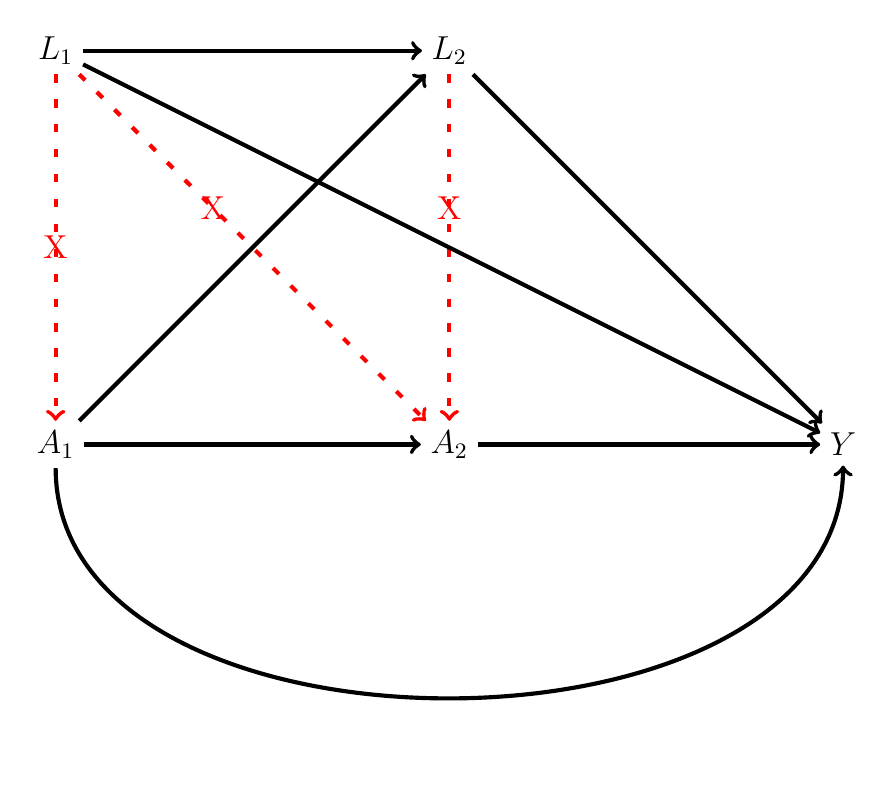
\begin{tikzpicture}
% nodes %
\node (L1) at (0, 0) {\large $L_{1}$};
\node (L2) at (5, 0) {\large $L_{2}$};
\node (A1) at (0, -5) {\large $A_{1}$};
\node (A2) at (5, -5) {\large $A_{2}$};
\node (Y) at (10, -5) {\large $Y$};
\node[red] at (0, -2.5) {\large X};
\node[red] at (5, -2) {\large X};
\node[red] at (2, -2) {\large X};
% edges %
\draw [->, line width= 1.5] (L1) -- (L2);
\draw [->, red, loosely dashed, line width= 1.5] (L1) -- (A1);
\draw [->, red, loosely dashed, line width= 1.5] (L1) -- (A2);
\draw [->, red, loosely dashed, line width= 1.5] (L2) -- (A2);
\draw [->, line width= 1.5] (A1) -- (A2);
\draw [->, line width= 1.5] (A1) to[out=-90,in=-90] (Y);
\draw [->, line width= 1.5] (A1) -- (L2);
\draw [->, line width= 1.5] (L1) -- (Y);
\draw [->, line width= 1.5] (A2) -- (Y);
\draw [->, line width= 1.5] (L2) -- (Y);
\end{tikzpicture}
\end{center}
\caption{The underlying logic of residual balancing: \(A_{t}\) denotes the
treatment at time \(t\), \(L_{t}\) is a vector of time-varying confounders
at time \(t\), and \(Y\) is the end-of-study outcome. Residual balancing weights break 
the confounding arrows \(L_{1}\rightarrow A_{1}\), \(L_{1}\rightarrow A_{2}\), and
\(L_{2}\rightarrow A_{2}\).}
\label{fig:1}
\end{figure}

\hypertarget{uses}{%
\section{Uses of residual balancing}\label{uses}}

The rationale described in the previous section is targeted at
estimating the causal effects of time-varying treatments. With minor
adaptations, we can expand the use of RBW to two other contexts commonly
encountered in the social and biomedical sciences: point treatment
situations and causal mediation analysis.

\hypertarget{rbw-treatment}{%
\subsection{RBW for estimating the average effect of a point
treatment}\label{rbw-treatment}}

RBW can be easily adapted to a point treatment situation where the user
aims only to adjust for a set of baseline (i.e., time-invariant)
confounders to estimate the average treatment effect. To this end, we
modify the procedure above as follows:

\begin{enumerate}
\def\labelenumi{\arabic{enumi}.}
\tightlist
\item
  Compute the response residuals \(\hat{\delta}(x_{ij})\) for each
  baseline confounder \(X_{j}\) by centering it around its sample mean:
  \(\hat{\delta}(x_{ij})=x_{ij}-\text{avg}({x}_{j})\).
\item
  Find a set of weights, \(rbw_{i}\), such that:

  \begin{enumerate}
  \def\labelenumii{\alph{enumii})}
  \tightlist
  \item
    in the weighted sample, the residuals \(\hat{\delta}(x_{ij})\) are
    orthogonal to the treatment;
  \item
    the relative entropy between \(rbw_{i}\) and the base weights
    \(q_{i}\) is minimized.
  \end{enumerate}
\item
  Use the weights to fit an MSM.
\end{enumerate}

The DAG of Figure \ref{fig:2} illustrates the point treatment situation.
\(A\) represents the one-shot treatment, \(X\) is a vector of baseline
confounders, and \(Y\) denotes our outcome. Weighting the observed
population by \(rbw_{i}\) mimics a pseudo-population where the link
between \(A\) and \(X\) is broken. We can then fit a model for the
conditional mean of \(Y\) given \(A\) to estimate the causal effects of
interest.\footnote{The vector \(X\) captures all confounding under the
  ignorability assumption.}

\begin{figure} [ht]
\begin{center}
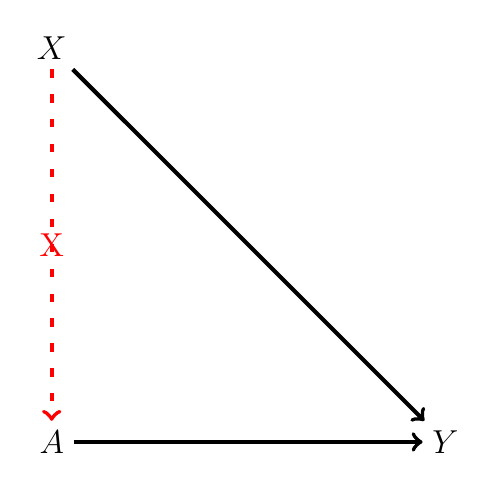
\begin{tikzpicture}
% nodes %
\node (A) at (0, 0) {\large $A$};
\node (Y) at (5, 0) {\large $Y$};
\node (X) at (0, 5) {\large $X$};
\node[red] at (0, 2.5) {\large X};
% edges %
\draw [->, line width= 1.5] (A) -- (Y);
\draw [->, red, loosely dashed, line width= 1.5] (X) -- (A);
\draw [->, line width= 1.5] (X) -- (Y);
\end{tikzpicture}
\end{center}
\caption{RBW in a point treatment: \(A\) represents the treatment,
\(X\) is a vector of baseline confounders, and \(Y\) denotes the outcome.
Residual balancing weights break the confounding arrow \(X\rightarrow A\).}
\label{fig:2}
\end{figure}

\hypertarget{rbw-mediation}{%
\subsection{RBW in causal mediation analysis}\label{rbw-mediation}}

In causal mediation analysis, researchers are often concerned with the
joint effects of a one-shot treatment, \(A\), and a mediator, \(M\), on
some end-of-study outcome \(Y\) when both baseline confounders (\(X\))
and some post-treatment confounders for the mediator-outcome
relationship (\(Z\)) are present. With minor adjustments, the RBW
implementation for causal mediation analysis is similar to the case with
time-varying treatments:

\begin{enumerate}
\def\labelenumi{\arabic{enumi}.}
\tightlist
\item
  As in the point treatment scenario, compute the response residuals
  \(\hat{\delta}(x_{ij})\) for each baseline confounder \(X_{j}\) by
  centering it around its sample mean.

  \begin{itemize}
  \tightlist
  \item
    Note: users may skip this step by including the baseline confounders
    in the MSM in the final step.
  \end{itemize}
\item
  Estimate the response residuals \(\hat{\delta}(z_{ij})\) for each
  post-treatment confounder \(Z_{j}\) by fitting a linear, logistic, or
  Poisson regression of \(z_{ij}\) (depending on its level of
  measurement) on the treatment \(a_{i}\) and the baseline confounders
  \(x_{i}\):
  \(\hat{\delta}(z_{ij})=z_{ij}-\mathbb{E}[z_{ij}|a_{i},x_{i}]\).
\item
  Find a set of weights, \(rbw_{i}\), such that:

  \begin{enumerate}
  \def\labelenumii{\alph{enumii})}
  \tightlist
  \item
    in the weighted sample, i) the baseline residuals
    \(\hat{\delta}(x_{ij})\) are orthogonal to the treatment \(a_{i}\)
    and the mediator \(m_{i}\); and ii) the post-treatment residuals
    \(\hat{\delta}(z_{ij})\) are balanced across the treatment
    \(a_{i}\), the mediator \(m_{i}\), and the baseline confounders
    \(x_{i}\);
  \item
    the relative entropy between \(rbw_{i}\) and the base weights
    \(q_{i}\) is minimized.
  \end{enumerate}
\item
  Use the weights to fit an MSM for the joint effects of the treatment
  and the mediator on the outcome:

  \begin{enumerate}
  \def\labelenumii{\alph{enumii})}
  \tightlist
  \item
    In causal mediation analysis, the potential outcomes of interest are
    denoted by \(Y(a,m)\) (this is the potential outcome under treatment
    \(a\) and mediator value \(m\)). We can then express a saturated MSM
    as
    \(\mathbb{E}[Y(a,m)]=\alpha_{0}+\alpha_{1}a+\alpha_{2}m+\alpha_{3}am\).
  \item
    Alternatively, the baseline confounders can be included in the MSM
    if users decide to skip the first step:
    \(\mathbb{E}[Y(a,m)|X]=\alpha_{0}+\alpha_{1}a+\alpha_{2}m+\alpha_{3}am+\alpha_{4}^{T}X\).
  \item
    Finally, the controlled direct effects (CDE) of the treatment can be
    estimated as
    \(\widehat{\text{CDE}}(m)=\mathbb{E}[Y(1,m)-Y(0,m)]=\hat{\alpha}_{1}+\hat{\alpha}_{3}m\).
    The CDE measures the causal effect of the treatment on the outcome
    when the mediator is fixed at some value \(m\) for all units.
  \end{enumerate}
\end{enumerate}

\hypertarget{r-package}{%
\section{The R package}\label{r-package}}

The R package \CRANpkg{rbw} contains four functions:

\begin{itemize}
\tightlist
\item
  \code{eb2()}, for generating minimum entropy weights subject to a set
  of balancing constraints.
\item
  \code{rbwPoint()}, for constructing residual balancing weights to
  estimate the causal effects of one-shot treatments.
\item
  \code{rbwMed()}, for constructing residual balancing weights to
  estimate controlled direct effects in causal mediation analysis.
\item
  \code{rbwPanel()}, for constructing residual balancing weights to
  estimate the marginal effects of time-varying treatments.
\end{itemize}

Next, we explain each of these functions. The package also includes
several real-world data sets (\code{advertisement}, \code{peace},
\code{campaign\_long}, and \code{campaign\_wide}), which we describe and
analyze in the examples below.

\hypertarget{eb2}{%
\subsection{\texorpdfstring{Function
\code{eb2()}}{Function }}\label{eb2}}

This function is an adaptation of \code{ebal::eb()} \citep{R-ebal}. It
is called internally by other functions in \CRANpkg{rbw} to implement
the method of Lagrange multipliers for locating a weighting solution
that minimizes the relative entropy between \(rbw_{i}\) and \(q_{i}\)
subject to the set of \(n_{c}\) balancing constraints described in
Equation \ref{eq:6}. \citet{zhouResidualBalancingMethod2020a} impose an
additional normalization constraint that ensures that the residual
balancing weights sum to the sample size: \(\sum_{i}rbw_{i}=n\).
Following \citet{hainmuellerEntropyBalancingCausal2012}, the authors
obtain the primal optimization problem:

\begin{equation}
\label{eq:8}
\min_{rbw_{i}}L^{p}=\sum^{n}_{i=1}rbw_{i}\log (rbw_{i}/q_{i})+\sum^{n_{c}}_{r=1}\lambda_{r}\sum^{n}_{i=1}rbw_{i}c_{ir}+\lambda_{0}\left(\sum^{n}_{i=1}rbw_{i}-n\right),
\end{equation}
where \(\{\lambda_{1},...,\lambda_{n_{c}}\}\) are the Lagrange
multipliers for the balancing constraints and \(\lambda_{0}\) is the
Lagrange multiplier for the normalization constraint. Since the loss
function \(L^{p}\) is strictly convex, the first order condition of
\(\frac{\partial L^{p}}{\partial rbw_{i}}=0\) implies that the solution
for each weight is

\begin{equation}
\label{eq:9}
rbw_{i}^{*}=\frac{nq_{i}\text{exp}(-\sum^{n_{c}}_{r=1}\lambda_{r}c_{ir})}{\sum^{n}_{i=1}q_{i}\text{exp}(-\sum^{n_{c}}_{r=1}\lambda_{r}c_{ir})}. 
\end{equation}

We can then insert Equation \ref{eq:9} into \(L^{p}\), leading to an
unrestricted dual problem:

\begin{equation}
\label{eq:10}
\max_{\lambda_{r}}L^{d}=-\log \left(\sum^{n}_{i=1}q_{i}\text{exp}\left(-\sum^{n_{c}}_{r=1}\lambda_{r}c_{ir}\right)\right),
\end{equation}
or equivalently,

\begin{equation}
\label{eq:11}
\min_{Z}L^{d}=\log \left(Q'\text{exp}(CZ)\right),
\end{equation}
where \(Q=[q_{1},...,q_{n}]'\),
\(C=[\boldsymbol{c}_{1},...,\boldsymbol{c}_{1}]'\), and
\(Z=-[\lambda_{1},...,\lambda_{n_{c}}]'\). Since \(L^{d}\) is strictly
convex, the solution is guaranteed to be unique --- assuming one exists.
Given that both the gradient and the Hessian have closed-form
expressions, we can solve the problem using Newton's method.
\code{eb2()} implements the algorithm. If convergence is successful, the
function tells the user that ``Entropy minimization converged within
tolerance level.'' Otherwise, it warns that entropy minimization did not
converge and suggests increasing the number of iterations or reducing
the number of balancing constraints.

The convexity of our optimization problem leads to appreciable
computational gains over other methods that use alternative loss
functions. This will be demonstrated later when we compare the
performance of RBW with that of npCBPS --- which uses the empirical
likelihood --- for the same problem.

\code{eb2()} is used as:

\code{eb2(C,\,M,\,Q,\,Z = rep(0,\,ncol(C)),\,max\_iter = 200,\,tol = 1e-04,\,print\_level = 1)}

and takes the following arguments:

\begin{itemize}
\tightlist
\item
  \code{C} is a constraint matrix, with each column corresponding to a
  balancing constraint.
\item
  \code{M} is a vector of moment conditions to be met in the reweighted
  sample (per Equation \ref{eq:6}, this is a vector of zeros with length
  equal to the number of columns of \texttt{C} when the other functions
  in \CRANpkg{rbw} call \texttt{eb2()} internally).
\item
  \code{Q} is a vector of base weights.
\item
  \code{Z} is a vector of Lagrange multipliers to be initialized.
\item
  \code{max\_iter} determines the maximum number of iterations for
  Newton's method.
\item
  \code{tol} is a tolerance parameter used to determine convergence.
  Specifically, convergence is achieved if \code{tol} is greater than
  the maximum absolute value of the deviations between the moments of
  the reweighted data and the target moments (i.e., \code{M}).
\item
  \code{print\_level} determines the level of printing:

  \begin{itemize}
  \tightlist
  \item
    \strong{1} normal: print whether the algorithm converges or not.
  \item
    \strong{2} detailed: print also the maximum absolute value of the
    deviations between the moments of the reweighted data and the target
    moments in each iteration.
  \item
    \strong{3} very detailed: print also the step length of the line
    searcher in iterations where a full Newton step is excessive.
  \end{itemize}
\end{itemize}

The output returned by \code{eb2()} is a list containing the following
elements:

\begin{itemize}
\tightlist
\item
  \code{W} is a vector of normalized minimum entropy weights.
\item
  \code{Z} is a vector of Lagrange multipliers.
\item
  \code{converged} is a logical indicator for convergence.
\item
  \code{maxdiff} is a scalar indicating the maximum absolute value of
  the deviation between the moments of the reweighted data and the
  target moments.
\end{itemize}

\hypertarget{rbwPoint}{%
\subsection{\texorpdfstring{Function
\code{rbwPoint()}}{Function }}\label{rbwPoint}}

This function produces residual balancing weights to be used in a point
treatment situation. It first takes a set of baseline confounders and
computes the residuals for each confounder by centering it around its
sample mean. Then it calls \code{eb2()} to find a set of weights,
\(rbw_{i}\), such that 1) the baseline residuals are orthogonal to the
treatment in the weighted sample, and 2) the relative entropy between
\({rbw}_{i}\) and the base weights is minimized. Additionally,
\code{rbwPoint()} calls a function that ensures that the matrix of
balancing constraints comprises only linearly independent columns.

\code{rbwPoint()} is used as:

\code{rbwPoint(treatment,\,data,\,baseline\_x,\,base\_weights,\,max\_iter = 200,}\\
\hspace*{0.333em}\hspace*{0.333em}\hspace*{0.333em}\hspace*{0.333em}\hspace*{0.333em}\hspace*{0.333em}\hspace*{0.333em}\hspace*{0.333em}\hspace*{0.333em}\hspace*{0.333em}\hspace*{0.333em}\code{tol = 1e-04,\,print\_level = 1)}

and takes the following arguments:

\begin{itemize}
\tightlist
\item
  \code{max\_iter}, \code{print\_level}, and \code{tol} have the same
  definitions as in \code{eb2()}.
\item
  \code{treatment} is a symbol or character string for the treatment
  variable.
\item
  \code{data} is a data frame containing all variables in the model.
\item
  \code{baseline\_x} is an expression for a set of baseline confounders
  stored in \code{data} or a character vector of the names of these
  variables.
\item
  \code{base\_weights} is an \emph{optional} vector of base weights (or
  its name). If no value is supplied, the function sets a vectors of
  ones with length equal to the sample size as the base weights.
\end{itemize}

The output returned by \code{rbwPoint()} is a list containing the
following elements:

\begin{itemize}
\tightlist
\item
  \code{weights} is a vector of residual balancing weights.
\item
  \code{constraints} is a matrix of linearly independent residual
  balancing constraints.
\item
  \code{eb\_out} contains the results from calling the \code{eb2()}
  function.
\item
  \code{call} is the matched call (the function call with all arguments
  specified by their full names).
\end{itemize}

\hypertarget{rbwMed}{%
\subsection{\texorpdfstring{Function
\code{rbwMed()}}{Function }}\label{rbwMed}}

This function produces residual balancing weights for causal mediation
analysis. It takes an \emph{optional} set of baseline confounders (as
explained above, users can opt instead to include these covariates in
the MSM later) and a list of model objects for the conditional mean of
each post-treatment confounder given the treatment and baseline
confounders. It then calls \code{eb2()} to find a set of weights,
\(rbw_{i}\), such that, in the weighted sample, 1) the baseline
residuals are orthogonal to the treatment and the mediator; 2) the
post-treatment confounders are balanced across the treatment, the
mediator, and the baseline confounders; and 3) the relative entropy
between \(rbw_{i}\) and the base weights is minimized.

\code{rbwMed()} takes an additional argument, \code{interact}, a logical
variable indicating whether the baseline and post-treatment confounders
should be balanced against the treatment-mediator interaction. This
argument is set to \code{FALSE} by default, but users suspecting an
interaction effect may find it prudent to balance against it. Like
\code{rbwPoint()}, \code{rbwMed()} calls a function internally to ensure
that only linearly independent columns constitute the matrix of
balancing constraints.

It is used as:

\code{rbwMed(treatment,\,mediator,\,zmodels,\,data,\,baseline\_x,\,interact = FALSE,}\\
\hspace*{0.333em}\hspace*{0.333em}\hspace*{0.333em}\hspace*{0.333em}\hspace*{0.333em}\hspace*{0.333em}\hspace*{0.333em}\hspace*{0.333em}\hspace*{0.333em}\hspace*{0.333em}\hspace*{0.333em}\code{base\_weights,\,max\_iter = 200,\,tol = 1e-04,\,print\_level = 1)}

and takes the following arguments:

\begin{itemize}
\tightlist
\item
  \code{treatment}, \code{data}, \code{base\_weights}, \code{max\_iter},
  \code{print\_level}, and \code{tol} are defined as in
  \code{rbwPoint()}.
\item
  \code{baseline\_x} is an \emph{optional} expression for a set of
  baseline confounders stored in \code{data} or a character vector of
  the names of these variables.
\item
  \code{mediator} is a symbol or character string representing the
  mediator variable.
\item
  \code{zmodels} is a list of fitted \code{lm} or \code{glm} objects for
  post-treatment confounders of the mediator-outcome relationship. Users
  should set this argument to \code{NULL} if there are no post-treatment
  confounders.
\item
  \code{interact} is a logical variable indicating whether baseline and
  post-treatment confounders should be balanced against the
  treatment-mediator interaction term(s).
\end{itemize}

The output returned by \code{rbwMed()} is a list containing the same
elements as the output from \code{rbwPoint()}.

\hypertarget{rbwPanel}{%
\subsection{\texorpdfstring{Function
\code{rbwPanel()}}{Function }}\label{rbwPanel}}

This function produces residual balancing weights for estimating the
marginal effects of time-varying treatments. It takes a list of model
objects for the conditional mean of each post-treatment confounder given
past treatments and past confounders. Then it calls \code{eb2()} to find
a set of weights, \(rbw_{i}\), such that 1) residuals of the
post-treatment confounders are orthogonal to future treatments and the
observed past in the weighted sample, and 2) the relative entropy
between \(rbw_{i}\) and the base weights is minimized. Like the other
functions, \code{rbwPanel()} ensures that the matrix of balancing
constraints consists only of linearly independent columns.

It is used as:

\code{rbwPanel(treatment,\,xmodels,\,id,\,time,\,data,\,base\_weights,\,future = 1L,}\\
\hspace*{0.333em}\hspace*{0.333em}\hspace*{0.333em}\hspace*{0.333em}\hspace*{0.333em}\hspace*{0.333em}\hspace*{0.333em}\hspace*{0.333em}\hspace*{0.333em}\hspace*{0.333em}\hspace*{0.333em}\code{max\_iter = 200,\,tol = 1e-04,\,print\_level = 1)}

and takes the following arguments:

\begin{itemize}
\tightlist
\item
  \code{data}, \code{base\_weights}, \code{max\_iter},
  \code{print\_level}, and \code{tol} are defined as in
  \code{rbwPoint()} and \code{rbwMed()}.
\item
  \code{treatment} is a symbol or character string for the time-varying
  treatment.
\item
  \code{xmodels} is a list of fitted \code{lm} or \code{glm} objects for
  time-varying confounders.
\item
  \code{id} is a symbol or character string for the unit id variable.
\item
  \code{time} is a symbol or character string for the time variable.
\item
  \code{future} is an integer indicating the number of future treatments
  in the balancing conditions. When \code{future > 0}, the residualized
  time-varying covariates are balanced not only with respect to current
  treatment \(A_{t}\), but also with respect to future treatments
  \(A_{t+1},...,A_{t+\texttt{future}}\). The default, \code{future = 1},
  assumes away higher-ordered lagged effects of the covariates on the
  treatment. Users can leave out lagged effects entirely by setting
  \code{future} to zero.
\end{itemize}

The output returned by \code{rbwPanel()} is essentially the same as
those from \code{rbwPoint()} and \code{rbwMed()}. The only difference is
that the \code{weights} object, instead of a vector, is now a data frame
with two columns: the id variable and the residual balancing weights
(the column storing the weights is called \code{rbw}).

\hypertarget{examples}{%
\section{Examples}\label{examples}}

We now illustrate the functions \code{rbwPoint()}, \code{rbwMed()}, and
\code{rbwPanel()} with data sets \code{advertisement}, \code{peace},
\code{campaign\_long}, and \code{campaign\_wide}, which are included in
\CRANpkg{rbw}. We expect users to rarely need to call \code{eb2()}
manually since its primary use is to be called internally by the other
functions. Hence, we see little gain in providing a separate example for
it.

\hypertarget{point-treatment-example}{%
\subsection{Point treatment: effects of political advertisements on
campaign contributions}\label{point-treatment-example}}

\citet{urbanDollarsSidewalkShould2014a} studied the effects of televised
political advertisements on campaign contributions. Presidential
candidates do not tend to deliberately advertise in states where
competition for electoral votes is tame. Yet, some areas of
noncompetitive states have overlapping media markets with battleground
states. Because these media market spillovers do not encompass other
forms of campaigning (e.g., rallies, speeches, etc.), the authors can
isolate the effect of television advertising by restricting their
analyses to noncompetitive states. Their original method involved
estimating the propensity score with a logistic model and then
conducting propensity score matching. To do so, they dichotomized the
political advertising variable to indicate whether a zip code received
more than 1000 advertisements.

Deeming this approach inadequate --- in part because balancing against a
dichotomous treatment does not ensure covariate balance on the
underlying continuous variable ---
\citet{fongCovariateBalancingPropensity2018} revisit the study using the
CBPS method applied to a continuous treatment. Next, we examine how RBW
fares compared with CBPS and IPW in this point treatment situation.

Importantly, CBPS assumes that the treatment variable is normally
distributed. To satisfy this assumption,
\citet{fongCovariateBalancingPropensity2018} search across Box-Cox
transformations to find the most appropriate transformation of the
treatment. Since Q-Q plots show no sizable differences between the
Box-Cox approach and a simple log transformation in achieving normality,
we favor the latter to avoid extraneous details that would divert the
example from its primary objective of illustrating RBW's implementation.
Hence, we have \(a_{i}^{*}=\log(a_{i}+1)\), where \(a_{i}\) is the
original treatment variable, the total number of political
advertisements in a zip code, and \(a_{i}^{*}\) is the transformed
treatment (we add one to \(a_{i}\) inside the log to avoid \(\log(0)\)
for zip codes receiving no advertisements). We also have a vector of
baseline confounders consisting of the zip code's log population,
population density, log median income, percent Hispanic, percent black,
percent over age 65, percent college graduates, and a binary indicator
of whether it is possible to commute to the zip code from a competitive
state. Finally, \(Y\) represents the outcome, campaign contributions in
thousands of dollars.

Our MSM includes the transformed treatment variable and state dummies
\(U\) to account for state fixed effects:

\begin{equation}
\label{eq:12}
\mathbb{E}[Y(a^{*})|U]=\theta_{0}+\theta_{1}a^{*} +\theta_{2}^{T}U.
\end{equation}

The data set \code{advertisement} contains the variables necessary for
the analyses. We start by loading the necessary packages and our data
set:

\begin{Schunk}
\begin{Sinput}
library("rbw")
data("advertisement")
\end{Sinput}
\end{Schunk}

\code{rbwPoint()} will construct the residual balancing weights by
following the steps described above. It first computes the baseline
residuals \(\hat{\delta}(x_{ij})=x_{ij}-\text{avg}({x}_{j})\) and then
finds a set of weights such that, in the weighted sample,
\(\hat{\delta}(x_{ij})\) are orthogonal to the treatment, and the
relative entropy between the residual balancing weights and a set of
base weights is minimized. Since \code{advertisement} does not include
sampling weights, \code{rbwPoint()} will set a vector of ones with
length equal to the sample size as the base weights.

\begin{Schunk}
\begin{Sinput}
rbwPoint_fit <-
  rbwPoint(
    treatment = treat,
    baseline_x = c(
      log_TotalPop,
      PercentOver65,
      log_Inc,
      PercentHispanic,
      PercentBlack,
      density,
      per_collegegrads,
      CanCommute
    ),
    data =
      advertisement
  )
\end{Sinput}
\end{Schunk}

Next, we attach the \(rbw_{i}\) weights to the data:

\begin{Schunk}
\begin{Sinput}
advertisement$rbwPoint_weights <- rbwPoint_fit$weights
\end{Sinput}
\end{Schunk}

Following most applications of MSMs, we compute standard errors using
the robust (``sandwich'') variance estimator. This can be implemented
with the function \code{survey::svydesign()}, which allows us to specify
a complex survey design and estimate standard errors consistent with
this specification.\footnote{\citet{zhouResidualBalancingMethod2020a}
  conduct a set of simulation studies to assess the performance of the
  robust variance estimator across different methods. They find that the
  estimator tends to overestimate the true sampling variance for
  residual balancing across nearly all scenarios, making it consistently
  conservative for RBW. By contrast, the estimator sometimes
  overestimates and other times underestimates the true sampling
  variance for other weighting methods, including CBPS.}

\begin{Schunk}
\begin{Sinput}
library("survey")
rbwPoint_design <- svydesign(ids = ~ 1,
                             weights = ~ rbwPoint_weights,
                             data = advertisement)
\end{Sinput}
\end{Schunk}

We then use the residual balancing weights to fit the MSM defined in
Equation \ref{eq:12}:

\begin{Schunk}
\begin{Sinput}
rbwPoint_msm <- svyglm(Cont ~ treat + factor(StFIPS),
                       design = rbwPoint_design)
\end{Sinput}
\end{Schunk}

Since we have transformed our treatment variable, we need to make the
necessary adjustments to compute the treatment effect. As
\citet{urbanDollarsSidewalkShould2014a} suggest, it is informative to
study the effect of going from zero to 1,000 political advertisements on
campaign contributions. Hence, we create a \code{dose} variable to
account for this. If \(a_{i}^{*}=\log(a_{i}+1)\), we can define our dose
as \(\log(1000+1)\):

\begin{Schunk}
\begin{Sinput}
dose <- log(1000 + 1)
\end{Sinput}
\end{Schunk}

To find the estimate \(\hat{\tau}_{rbw}\) of the average treatment
effect, we multiply the coefficient for the transformed treatment
variable by our dose. We also multiply it by 1,000 since the outcome
variable is measured in thousands of dollars:

\begin{Schunk}
\begin{Sinput}
rbwPoint_tau <- 1000 * coef(rbwPoint_msm)[2] * dose
\end{Sinput}
\end{Schunk}

Next, we use the basic properties of the variance operator to derive the
standard error. Again, we multiply the result by 1,000 given the scale
of the outcome variable:

\begin{Schunk}
\begin{Sinput}
rbwPoint_vcov <- stats::vcov(rbwPoint_msm)
rbwPoint_se <- 1000 * dose * sqrt(rbwPoint_vcov[2, 2]) 
\end{Sinput}
\end{Schunk}

We also report the results using the functions from the \CRANpkg{CBPS}
and \CRANpkg{ipw} packages. Recall from the introduction that the
parametric CBPS is similar to IPW in that it requires explicit models
for the conditional distributions of the treatment. However, it improves
IPW by considering a set of balancing conditions during the propensity
score estimation, thereby reducing sensitivity to model
misspecification. By contrast, the nonparametric CBPS (npCBPS) does not
require direct estimation of the propensity score; instead, it finds
weights that maximize the empirical likelihood while meeting a set of
balancing constraints. As such, like RBW, it avoids the need to specify
a propensity score model. Readers can find the code detailing the
construction of the CBPS and IPW weights in the supplementary material.

Table \ref{tab:point-treatment-comparison} summarizes the findings. All
methods yield relatively similar point estimates and standard errors. In
particular, they indicate that going from zero to 1,000 political
advertisements increases campaign contributions by around four thousand
dollars, on average, although the point estimates from CBPS and IPW are
slightly larger than those produced by RBW and npCBPS. The last column
shows that different loss functions for the optimization problem can
lead to stark differences in computation time. While RBW's relative
entropy metric leads to a convex optimization problem that Newton's
method can solve in less than one second, npCBPS's algorithm takes much
longer to run.

\begin{Schunk}
\begin{table}[ht]

\caption{\label{tab:point-treatment-comparison}Comparison of RBW, npCBPS, CBPS, and IPW for a Point Treatment Situation}
\centering
\begin{tabular}[t]{lccc}
\toprule
Method & Estimate & Standard Error & Computation Time (in Seconds)\\
\midrule
RBW & 4043 & 2131 & 0.51\\
npCBPS & 3914 & 2091 & 118.70\\
CBPS & 4181 & 2118 & 7.71\\
IPW & 4118 & 2078 & 0.04\\
\bottomrule
\multicolumn{4}{l}{\textsuperscript{} Computation time may differ depending on system setup.}\\
\multicolumn{4}{l}{\textsuperscript{} System setup used to generate the results:}\\
\multicolumn{4}{l}{\textsuperscript{} MacBook Pro (15-inch, 2018), 2.2 GHz 6-Core Intel Core i7, 16GB RAM.}\\
\end{tabular}
\end{table}

\end{Schunk}

We next illustrate the use of \code{rbwMed()} and \code{rbwPanel()}.

\hypertarget{causal-mediation-example}{%
\subsection{Causal mediation analysis: the controlled direct effect of
shared democracy on public support for
war}\label{causal-mediation-example}}

A stylized fact in political science is that democracies do not engage
in war with one another. To assess the role of public opinion in keeping
the peace, \citet{tomzPublicOpinionDemocratic2013a} designed survey
experiments that presented participants with a situation where a country
was developing nuclear weapons. When describing the situation, the
authors randomly and independently changed three characteristics of the
country: its political regime (whether it was a democracy), alliance
status (whether it had signed a military alliance with the United
States), and economic ties (whether it had high levels of trade with the
US). The outcome of interest was the respondent's support for military
action on a five-point scale ranging from ``oppose strongly'' to ``favor
strongly.'' The authors found that respondents were considerably less
supportive of military action against democracies than otherwise
identical autocratic regimes.

\citet{tomzPublicOpinionDemocratic2013a} then went on to investigate the
causal mechanisms through which shared democracy reduces public
enthusiasm for war. In particular, they measured individuals' beliefs
about the level of threat posed by the potential adversary (number of
adverse events respondents considered probable if the US did not engage
in war); the cost of the intervention (number of negative consequences
anticipated if the US engaged in war); and the likelihood of success (a
three-point scale assigning values of 0, 1, and 2 to the following
beliefs, respectively: the operation had less than a 50-50 chance of
working even in the short run, it would succeed only in the short run,
and it would be successful both in the short and long run). They also
collected data on people's moral concerns about using military force.

Their methodological framework focused on estimating the natural direct
and natural indirect effects
\citep{imaiUnpackingBlackBox2011, imaiIdentificationInferenceSensitivity2010},
whose identification assumptions require that no post-treatment
confounding of the mediator-outcome relationship exists. As such, the
authors examined the role of each mediator separately by assuming they
operate independently of one another. Yet, as discussed in
\citet{zhouResidualBalancingMethod2020a}, beliefs about the threat,
cost, and likelihood of success may affect an individual's perceptions
of morality while also influencing support for war directly. By treating
these variables as post-treatment confounders,
\citet{zhouResidualBalancingMethod2020a} analyzed the mediating role of
morality using controlled direct effects.

Let \(A\) denote the treatment, whether the country developing nuclear
weapons was presented as a democracy, \(M\) the mediator, a dummy
variable indicating whether the participant deemed the military action
morally wrong, and \(Y\) the outcome, the respondent's support for war
on a five-point scale. We also have a set of baseline confounders
(\(X\)) including dummies for the other two randomized treatments
(alliance status and economic ties) in addition to several demographic
and attitudinal controls.\footnote{For example, attitudinal controls
  include respondents' attitudes toward ethnocentrism measured with a
  series of questions about their opinions on immigration, affirmative
  action, and gay marriage.} Finally, \(Z\) is the vector of
post-treatment confounders comprising measures of beliefs about the
threat, cost, and likelihood of success.

Our MSM is thus defined as:

\begin{equation}
\label{eq:13}
\mathbb{E}[Y(a, m)]=\alpha_{0}+\alpha_{1}a +\alpha_{2}m+\alpha_{3}am.
\end{equation}

We can alternatively include the baseline confounders in the MSM instead
of balancing them across the treatment and the mediator with baseline
residuals:

\begin{equation}
\label{eq:14}
\mathbb{E}[Y(a, m)|X]=\alpha_{0}+\alpha_{1}a +\alpha_{2}m+\alpha_{3}am + \alpha_{4}^{T}X.
\end{equation}

The \code{peace} data set includes the variables we will use in the
analyses. Let us first consider the approach where the baseline
confounders are balanced across the treatment and the mediator using the
baseline residuals computed from centering each covariate around its
sample mean.

As explained above, RBW in causal mediation analysis requires models for
the conditional means of each post-treatment confounder \(Z_{j}\) given
the treatment \(a_{i}\) and the baseline confounders \(x_{i}\):
\(\hat{\mathbb{E}}[z_{ij}|a_{i},x_{i}]\). Hence, we assume that
\code{threatc}, \code{cost}, and \code{successc} are measured on a
continuous scale and fit linear models for each:

\begin{Schunk}
\begin{Sinput}
data("peace")
z1 <- lm(threatc ~ ally + trade + h1 + i1 + p1 + e1 + r1 +
           male + white + age + ed4 + democ,
         data = peace)
z2 <- lm(cost ~ ally + trade + h1 + i1 + p1 + e1 + r1 +
           male + white + age + ed4 + democ,
         data = peace)
z3 <- lm(successc ~ ally + trade + h1 + i1 + p1 + e1 + r1 +
           male + white + age + ed4 + democ,
         data = peace)
\end{Sinput}
\end{Schunk}

We then store the three model objects together in a list to be passed
later to the \code{zmodels} argument in \code{rbwMed()}:

\begin{Schunk}
\begin{Sinput}
zmodels <- list(z1, z2, z3)
\end{Sinput}
\end{Schunk}

To construct the residual balancing weights, \code{rbwMed()} will 1)
compute the baseline residuals
\(\hat{\delta}(x_{ij})=x_{ij}-\text{avg}({x}_{j})\) and the
post-treatment residuals
\(\hat{\delta}(z_{ij})=z_{ij}-\mathbb{E}[z_{ij}|a_{i},x_{i}]\) and 2)
find a set of weights such that a) in the weighted sample, the baseline
and post-treatment residuals meet the orthogonality requirements
described earlier, and b) the relative entropy between the residual
balancing weights and a set of base weights is minimized. The function
will use a vector of ones as the base weights since \code{peace} does
not include sampling weights. We also pass the name of our mediator to
the \code{mediator} argument:

\begin{Schunk}
\begin{Sinput}
rbwMed_fit <- rbwMed(
  treatment = democ,
  mediator = immoral,
  zmodels = zmodels,
  baseline_x = c(ally, trade, h1, i1,
                 p1, e1, r1, male, white, age, ed4),
  data = peace
)
\end{Sinput}
\begin{Soutput}
#> Entropy minimization converged within tolerance level
\end{Soutput}
\end{Schunk}

Next, we attach the weights to \code{peace}:

\begin{Schunk}
\begin{Sinput}
peace$rbwMed_weights <- rbwMed_fit$weights
\end{Sinput}
\end{Schunk}

We use \code{survey::svydesign()} to estimate robust standard errors:

\begin{Schunk}
\begin{Sinput}
rbwMed_design <- svydesign(ids = ~ 1,
                           weights = ~ rbwMed_weights,
                           data = peace)
\end{Sinput}
\end{Schunk}

Finally, we use the residual balancing weights to fit the MSM from
Equation \ref{eq:13}:

\begin{Schunk}
\begin{Sinput}
rbwMed_msm <- svyglm(strike ~ democ * immoral,
                     design = rbwMed_design)
\end{Sinput}
\end{Schunk}

Steps are similar for the case where the baseline confounders are not
balanced against the treatment and the mediator but instead adjusted in
the MSM, as defined in Equation \ref{eq:14}. The models for the
conditional means of the post-treatment confounders are the same as
before, but we now leave the \code{baseline\_x} argument empty:

\begin{Schunk}
\begin{Sinput}
rbwMed2_fit <- rbwMed(
  treatment = democ,
  mediator = immoral,
  zmodels = zmodels,
  data = peace
)
\end{Sinput}
\begin{Soutput}
#> Entropy minimization converged within tolerance level
\end{Soutput}
\begin{Sinput}
peace$rbwMed2_weights <- rbwMed2_fit$weights
rbwMed2_design <- svydesign(ids = ~ 1,
                            weights = ~ rbwMed2_weights,
                            data = peace)
rbwMed2_msm <- svyglm(strike ~ ally + trade + h1 + i1 + p1 +
                        e1 + r1 + male + white + age + ed4 + democ * immoral,
                      design = rbwMed2_design)
\end{Sinput}
\end{Schunk}

We summarize the results in Table \ref{mediation-comparison}. The
estimated CDE if respondents lacked any moral qualms about military
intervention, i.e.,
\(\widehat{\text{CDE}}(m=0)=\hat{\mathbb{E}}[Y(1,0)-Y(0,0)]=\hat{\alpha}_{1}\),
is \(-0.32\) under the first approach and \(-0.36\) under the second.
Both estimates are statistically significant at the level of 0.01. The
estimated CDE if respondents had moral qualms about military
intervention, i.e.,
\(\widehat{\text{CDE}}(m=1)=\hat{\mathbb{E}}[Y(1,1)-Y(0,1)]=\hat{\alpha}_{1} + \hat{\alpha}_{3}\),
is \(-0.36\) under the first approach and \(-0.22\) under the second.

\begin{table}[ht] \centering 
  \caption{MSM Results for the Controlled Direct Effects of Shared Democracy on Public Support for War:
  \(\widehat{\text{CDE}}(m=0)\) Equals the Coefficient for Shared Democracy;
  \(\widehat{\text{CDE}}(m=1)\) Equals the Coefficient for Shared Democracy Plus the Coefficient for
  the Interaction Term} 
  \label{mediation-comparison} 
\begin{tabular}{@{\extracolsep{5pt}}lcc} 
\\[-1.8ex]\toprule 
 & \shortstack{Baseline Confounders \\ Balanced} & \shortstack{Baseline Confounders \\ Adjusted in the MSM} \\
\midrule
 Shared democracy & $-$0.317$^{***}$ & $-$0.360$^{***}$ \\ 
  & (0.098) & (0.080) \\ 
  & & \\ 
 Moral concerns & $-$1.272$^{***}$ & $-$1.201$^{***}$ \\ 
  & (0.175) & (0.135) \\ 
  & & \\ 
 Shared democracy * Moral concerns & $-$0.048 & 0.138 \\ 
  & (0.210) & (0.157) \\ 
\bottomrule \\[-1.8ex] 
\multicolumn{3}{l}{$^{*}$p$<$0.1; $^{**}$p$<$0.05; $^{***}$p$<$0.01} \\ 
\multicolumn{3}{l}{Robust standard errors in parentheses.} \\ 
\end{tabular} 
\end{table}

\hypertarget{time-varying-example}{%
\subsection{Time-varying treatment: the cumulative effect of negative
advertising on vote shares}\label{time-varying-example}}

We conclude this section with an example of RBW applied to a context
involving time-varying treatments and confounders. Political scientists
have shown interest in examining the cumulative effect of negative
campaign advertising on election outcomes
\citep{lauEffectsNegativePolitical2007, blackwellFrameworkDynamicCausal2013, imaiRobustEstimationInverse2015}.
This is an intricate process because while polling results affect
current campaign strategies, they are also constantly shifting, as they
respond both to previous results and candidates' use of negative
advertising in the past. For their ability to accommodate dynamic causal
relationships --- particularly since they allow past treatments to
affect current outcomes (i.e., ``carryover effects'') and past outcomes
to influence current treatment (i.e., ``feedback effects'')
\citep{imaiWhenShouldWe2019} --- MSMs are suitable for this research
question.

We use a dataset on the campaign of 113 Democratic candidates in US
Senate and Gubernatorial Elections from 2000 to 2006. Let \(A_{t}\)
represent our continuous treatment, the proportion of campaign
advertisements mentioning the adversary in each campaign week, \(L_{t}\)
our time-varying confounders, the Democratic share and the share of
undecided voters in the polls, and \(Y\) the outcome, the Democratic
share of the two-party vote. Additionally, we have a set of baseline
confounders \(X\) including total campaign length, election year, and
whether the election is senatorial or gubernatorial.

\citet{zhouResidualBalancingMethod2020a} define an MSM as follows:

\begin{equation}
\label{eq:15}
\mathbb{E}[Y(\bar{a})|X]=\beta_{0}+\beta_{1}\text{avg}(\bar{a})+\beta_{2}V+\beta_{3}\text{avg}(\bar{a})V+\beta_{4}^{T}X,
\end{equation}
where \(V\) is an indicator of incumbency status used to construct
interactions that allow the effect to differ between incumbents and
nonincumbents, and \(\text{avg}(\bar{a})\) is the average proportion of
advertisements that were negative over the final five weeks of the
campaign multiplied by ten (following
\citet{zhouResidualBalancingMethod2020a}, we multiply this quantity by
ten so that the regression coefficients can be interpreted as the effect
of a ten-percentage point increase in negative advertising).

\CRANpkg{rbw} contains two data sets associated with this problem:
\code{campaign\_long} and \code{campaign\_wide}. They represent,
respectively, the long-format and wide-format data on negative campaign
advertising.

Recall that RBW requires us to fit a model for the conditional mean of
each covariate at each time point given the observed past. We thus
estimate regression models of our time-varying confounders \(L_{t}\)
(\(t\ge2\)) on lagged treatment and lagged confounders. We also interact
each regressor with the week dummies, thus allowing the coefficients to
change over time in a flexible manner:

\begin{Schunk}
\begin{Sinput}
data("campaign_long")
data("campaign_wide")
x1 <-
  lm(dem.polls ~ (neg.dem.l1 + dem.polls.l1 + undother.l1) * factor(week),
     data = campaign_long)
x2 <-
  lm(undother ~ (neg.dem.l1 + dem.polls.l1 + undother.l1) * factor(week),
     data = campaign_long)
\end{Sinput}
\end{Schunk}

We then create a list with the model objects to be passed later to the
\code{xmodels} argument in \code{rbwPanel()}:

\begin{Schunk}
\begin{Sinput}
xmodels <- list(x1, x2)
\end{Sinput}
\end{Schunk}

To construct the residual balancing weights, \code{rbwPanel()} first
extracts the residual terms \(\hat{\delta}(L_{t})\) from the models
above. Note that for each covariate in \(L_{1}\) (the first time
period), the residuals are computed as deviations from the sample mean.
Then the function finds a set of weights, such that, in the weighted
sample, the residuals are orthogonal to current and future treatments as
well as the regressors of \(L_{jt}\), and the relative entropy between
the residual balancing weights and the base weights is minimized. Note
that we set the \code{future} argument to zero to replicate the results
from \citet{zhouResidualBalancingMethod2020a} since the authors balance
the residualized time-varying confounders only with respect to the
current treatment, thus assuming away lagged effects of the covariates
on the treatment.\footnote{The negative advertising data set spans five
  weeks, so lagged effects of the time-varying covariates on the
  treatment can be incorporated by setting \code{future > 0}, up to
  \code{future = 4}.} Since our data do not include sampling weights, a
vector of ones is used as the base weights. Additionally, we need to
pass arguments indicating the unit id and the time variables due to the
longitudinal structure of our data set.

\begin{Schunk}
\begin{Sinput}
rbwPanel_fit <- rbwPanel(
  treatment = neg.dem,
  xmodels = xmodels,
  id = id,
  time = week,
  data = campaign_long,
  future = 0
)
\end{Sinput}
\begin{Soutput}
#> Entropy minimization converged within tolerance level
\end{Soutput}
\end{Schunk}

We now attach the weights to \code{campaign\_wide} using the pipe
operator and the \code{left\_join()} function from the package
\CRANpkg{dplyr} (this merging is permitted because the \code{weights}
object returned by \code{rbwPanel()} is a data frame containing the id
variable and the residual balancing weights):

\begin{Schunk}
\begin{Sinput}
library("dplyr")
campaign_wide <- campaign_wide %>%
  left_join(rbwPanel_fit$weights, by = "id")
\end{Sinput}
\end{Schunk}

We use the functions from \CRANpkg{dplyr} to rename the weights so that
our variable's name is consistent with the previous examples:

\begin{Schunk}
\begin{Sinput}
campaign_wide <- campaign_wide %>%
  rename(rbwPanel_weights = rbw)
\end{Sinput}
\end{Schunk}

Again, we use \code{survey::svydesign()} to compute robust standard
errors:

\begin{Schunk}
\begin{Sinput}
rbwPanel_design <- svydesign(ids = ~ 1,
                             weights = ~ rbwPanel_weights,
                             data = campaign_wide)
\end{Sinput}
\end{Schunk}

Finally, we use the residual balancing weights to fit the MSM from
Equation \ref{eq:15}:

\begin{Schunk}
\begin{Sinput}
rbwPanel_msm <- svyglm(demprcnt ~ ave_neg * deminc + camp.length +
                         factor(year) + office,
                       design = rbwPanel_design)
\end{Sinput}
\end{Schunk}

We report the model results in Table \ref{time-varying-model}. The
estimate for nonincumbents is \(0.49\) and for incumbents is
\(0.49-1.48=-0.99\). The effect of negative advertisement for
nonincumbents is positive though not statistically significant --- a ten
percentage point increase in the proportion of negative advertising
throughout the last five weeks of the campaign increases the Democratic
vote share by about half a percentage point, on average. However, the
interaction term is significant at the level of 0.01, and incumbents see
a sizeable negative effect from negative advertising: a ten percentage
point increase in negative advertising reduces a candidate's vote share
by about one percentage point, on average.

\begin{table}[ht] \centering 
  \caption{MSM Results for the Cumulative Effect of Negative Advertising on Vote Shares} 
  \label{time-varying-model} 
\begin{tabular}{@{\extracolsep{5pt}}lc} 
\\[-1.8ex]\toprule
 Average proportion & 0.490 \\ 
  & (0.315) \\ 
  & \\ 
 Incumbency & 14.971$^{***}$ \\ 
  & (2.823) \\ 
  & \\ 
 Average proportion * Incumbency & $-$1.484$^{***}$ \\ 
  & (0.531) \\ 
\bottomrule \\[-1.8ex] 
\multicolumn{2}{l}{$^{*}$p$<$0.1; $^{**}$p$<$0.05; $^{***}$p$<$0.01} \\ 
\multicolumn{2}{l}{Robust standard errors in parentheses.} \\ 
\end{tabular} 
\end{table}

We conclude by comparing RBW's computational performance to CBPS for a
dichotomized version of the treatment representing whether more than
10\% of the candidate's advertising was negative for each week. We use
this dichotomized variable because CBPS has not been extended to work
with continuous treatments in longitudinal settings. Additionally, we do
not compare RBW to npCBPS because the latter's use is restricted to
point treatment situations. Lastly, though we can construct IPW weights
almost immediately, \citet{zhouResidualBalancingMethod2020a} show that
IPW yields considerably larger effect estimates than RBW and CBPS for
this particular case (likely due to the method's susceptibility to model
misspecification), so we do not report the IPW results.

Let us first construct the RBW weights. The steps are identical to the
ones detailed above for the continuous treatment, the only change being
the name of our treatment variable. Next, we use the \code{CBMSM()}
function from the \code{CBPS} package to generate our CBPS weights. To
facilitate comparisons of computation time, we also call
\code{Sys.time()} before and after running the functions that produce
the weights in each package. The scalar objects \code{rbwPanel\_time}
and \code{CBPSPanel\_time} store how long each method takes to construct
the corresponding weights.

\begin{Schunk}
\begin{Sinput}
m1 <-
  lm(dem.polls ~ (d.gone.neg.l1 + dem.polls.l1 + undother.l1) * factor(week),
     data = campaign_long)
m2 <-
  lm(undother ~ (d.gone.neg.l1 + dem.polls.l1 + undother.l1) * factor(week),
     data = campaign_long)

xmodels <- list(m1, m2)

rbwPanel_start <- Sys.time()
rbwPanel_fit <- rbwPanel(
  treatment = d.gone.neg,
  xmodels = xmodels,
  id = id,
  time = week,
  data = campaign_long,
  future = 0
)
\end{Sinput}
\begin{Soutput}
#> Entropy minimization converged within tolerance level
\end{Soutput}
\begin{Sinput}
rbwPanel_end <- Sys.time()
rbwPanel_time <- rbwPanel_end - rbwPanel_start
\end{Sinput}
\end{Schunk}

\begin{Schunk}
\begin{Sinput}
CBPSPanel_form <-
  "d.gone.neg ~ d.gone.neg.l1 + dem.polls + undother + camp.length + deminc + office + factor(year)"

CBPSPanel_start <- Sys.time()
CBPSPanel_fit <-
  CBMSM(
    formula = CBPSPanel_form,
    time = campaign_long$week,
    id = campaign_long$demName,
    data = campaign_long,
    type = "MSM",
    iterations = NULL,
    twostep = TRUE,
    msm.variance = "approx",
    time.vary = TRUE
  )
CBPSPanel_end <- Sys.time()
CBPSPanel_time <- CBPSPanel_end - CBPSPanel_start
\end{Sinput}
\end{Schunk}

The output below shows the computation times:

\begin{Schunk}
\begin{Sinput}
rbwPanel_time
\end{Sinput}
\begin{Soutput}
#> Time difference of 0.107008 secs
\end{Soutput}
\begin{Sinput}
CBPSPanel_time
\end{Sinput}
\begin{Soutput}
#> Time difference of 1.059287 mins
\end{Soutput}
\end{Schunk}

Whereas RBW takes less than one second to construct the weights, CBPS
takes much longer. Hence, the longitudinal setting presents the same
pattern we saw above for the point treatment situation: RBW has
considerable gains in computational performance over alternative methods
of constructing weights for MSMs. Since our focus here is computational
performance, we omit the effect estimates for the dichotomized
treatment. As shown in \citet{zhouResidualBalancingMethod2020a}, the
results are broadly consistent with those based on the continuous
treatment, with RBW and CBPS yielding similar point estimates.

\hypertarget{conclusion}{%
\section{Conclusion}\label{conclusion}}

Compared to other methods of constructing weights for MSMs, RBW has
several advantages. In particular, it does not require modeling the
conditional distributions of exposures and is thus easy to use with
continuous treatments. Previous simulation studies suggest that it is
often more efficient and more robust to model misspecification than
alternative weighting strategies
\citep{zhouResidualBalancingMethod2020a}. RBW is also favorable from a
computational perspective. Its procedure for finding weights involves a
convex optimization problem, allowing RBW to locate a solution
substantially faster than alternative methods whose optimization relies
on nonconvex loss functions --- such as the recently proposed
nonparametric version of CBPS, which uses the empirical likelihood
\citep{fongCovariateBalancingPropensity2018}. Table
\ref{tab:method-comparison} sums up these comparisons.

\begin{table}[ht]

\caption{\label{tab:method-comparison}Comparison of Methods and Software Implementation}
\centering
\begin{tabular}[t]{ccccc}
\toprule
Method & \makecell[c]{Models for\\Conditional Distributions of\\Exposures} & \makecell[c]{Balancing\\Constraints} & \makecell[c]{Implemented for\\Time-varying\\Treatments?} & R Package\\
\midrule
IPW & Required & Absent & Yes & \pkg{ipw}\\
CBPS & Required & Present & Yes & \pkg{CBPS}\\
npCBPS & Not Required & Present & No & \pkg{CBPS}\\
RBW & Not Required & Present & Yes & \pkg{rbw}\\
\bottomrule
\end{tabular}
\end{table}

After explaining the underlying logic of RBW, we have described its
implementation in the R package \CRANpkg{rbw}. With examples from
several data sets, we have demonstrated the use of \CRANpkg{rbw} in
three distinct contexts: effect estimation for point treatments, causal
mediation analysis, and effect estimation for time-varying treatments
with time-varying confounders.

Nonetheless, RBW is not without limitations. In particular, it depends
on models for the conditional means of post-treatment confounders. When
these models are incorrectly specified, the pseudo-population generated
by residual balancing weights will fail to mimic the original unweighted
population, and our estimates will be biased. Even when these models are
correctly specified, RBW may also yield biased estimates when we have
insufficient balancing conditions. Adding more functions such as
cross-products and high-order terms to the set
\(G(L_{t})=\{g_{1}(L_{t}),...,g_{J_{t}}(L_{t})\}\), thereby increasing
the number of balancing constraints, may help --- though at the risk of
making exact balance infeasible. Future work may extend RBW to allow for
approximate balance with a penalty for the remaining imbalance in the
optimization problem \citep{fongCovariateBalancingPropensity2018}.
Finally, we have relied on the ``sandwich'' variance estimator to
compute standard errors. Though \citet{zhouResidualBalancingMethod2020a}
demonstrate with simulation studies that this estimator is likely
conservative for RBW, they do not provide a variance estimator tailored
to address the estimation uncertainty of the RBW weights.

Despite these limitations, RBW will be useful to many social scientists
interested in using marginal structural models to study causality in
dynamic settings. We will continue to upgrade the package by expanding
RBW's ranges of applicability --- specifically, to censored data, to
contexts involving repeated outcome measures including survival data
\citep{hernanMarginalStructuralModels2000, hernanEstimatingCausalEffect2002},
and to cases where, as discussed above, exact balance is infeasible and
approximate balance must be pursued.

\hypertarget{acknowledgments}{%
\section{Acknowledgments}\label{acknowledgments}}

We thank Geoffrey Wodtke and two anonymous reviewers for their valuable
comments on a previous version of this paper.

\bibliography{baum-zhou-final.bib}

\address{%
Derick S. Baum\\
Harvard University\\%
Department of Sociology\\
%
%
%
\href{mailto:derick_baum@g.harvard.edu}{\nolinkurl{derick\_baum@g.harvard.edu}}%
}

\address{%
Xiang Zhou\\
Harvard University\\%
Department of Sociology\\
%
%
%
\href{mailto:xiang_zhou@fas.harvard.edu}{\nolinkurl{xiang\_zhou@fas.harvard.edu}}%
}
